\chapter{系统实现}
\label{cha:systemRealize}

系统是如何实现的?

\section{一些关键技术实现方案}

\subsection{怎么怎么样}

xxxx

\subsubsection{这样这样}

如果更详细的划分

表格什么的

\begin{table}[htbp] 
  \centering
    \caption{\label{tab:touch}触摸事件类型\cite{cccManual}} 
    \begin{tabular}{lcl} 
      \toprule[1.5pt]
      {\heiti 枚举对象定义} & {\heiti 时间名} & {\heiti 触发时机} \\\midrule[1pt]
      % \midrule 
      cc.Node.EventType.TOUCH\_START &	touchstart &	当手指触点落在目标节点区域内时  \\
      cc.Node.EventType.TOUCH\_MOVE &	touchmove &	当手指在屏幕上目标节点区域内移动时  \\
      cc.Node.EventType.TOUCH\_END &	touchend &	当手指在目标节点区域内离开屏幕时  \\
      cc.Node.EventType.TOUCH\_CANCEL &	touchcancel &	当手指在目标节点区域外离开屏幕时  \\
      \bottomrule[1.5pt]
    \end{tabular} 
\end{table}

如果想要插入代码

\textbf{Example:}
\begin{lstlisting}[escapeinside=``, basicstyle=\small, breaklines]
  node.on(cc.Node.EventType.MOUSE_DOWN, function (event) {
    console.log('Mouse down');
  }, this);
\end{lstlisting}

\section{还有啥}

\subsection{xx官网}

双图

xx官网界面如图 \ref{fig:gameWeb} 所示。

\begin{figure}[h]
  \centering%
  \subcaptionbox{官网主页\label{fig:gameWeb}} %标题的长度,超过则会换行,如下一个小图。
    {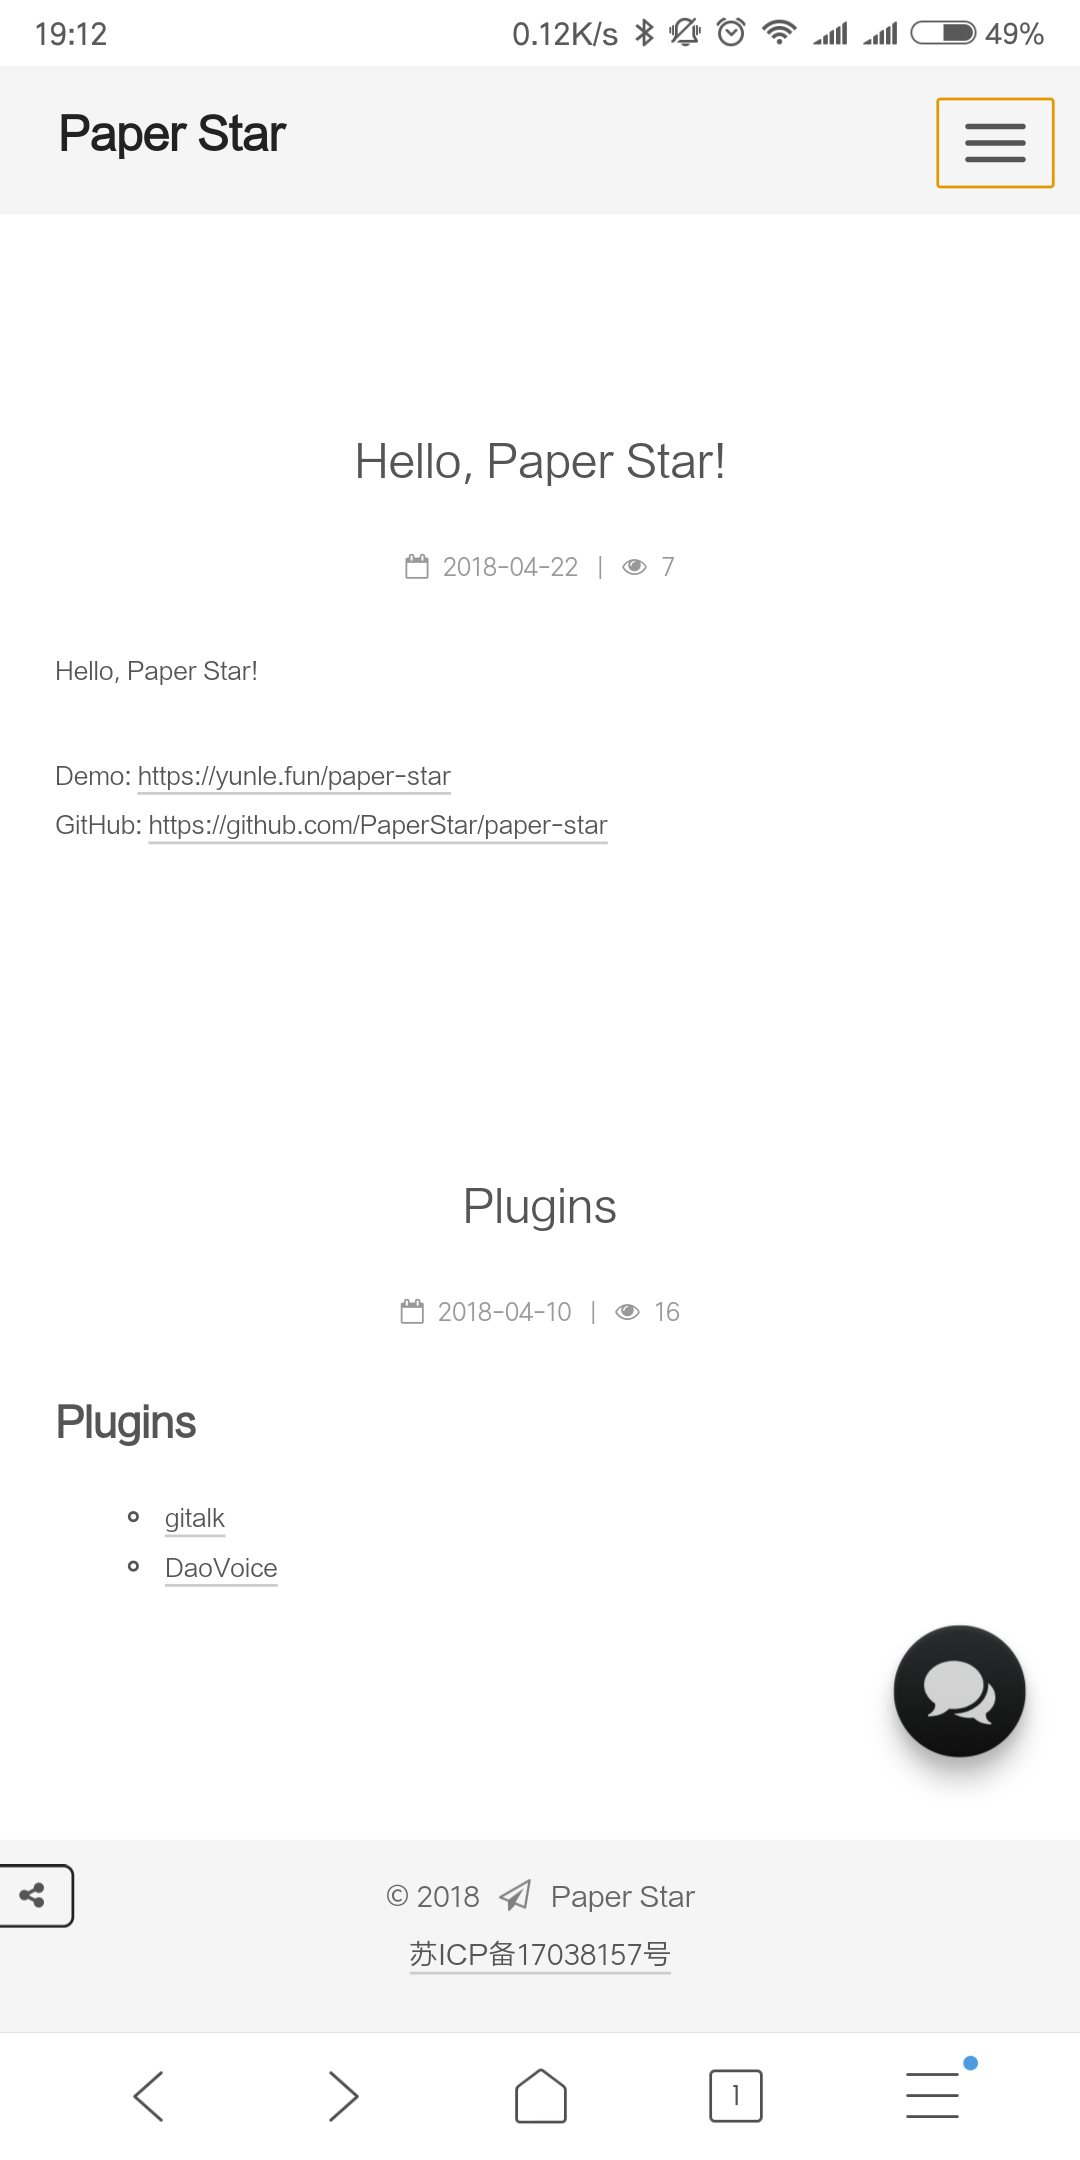
\includegraphics[width=5cm]{show/gameWeb-main}}%
  \hspace{4em}%
  \subcaptionbox{文章评论\label{fig:gameWeb-gitalk}}
      {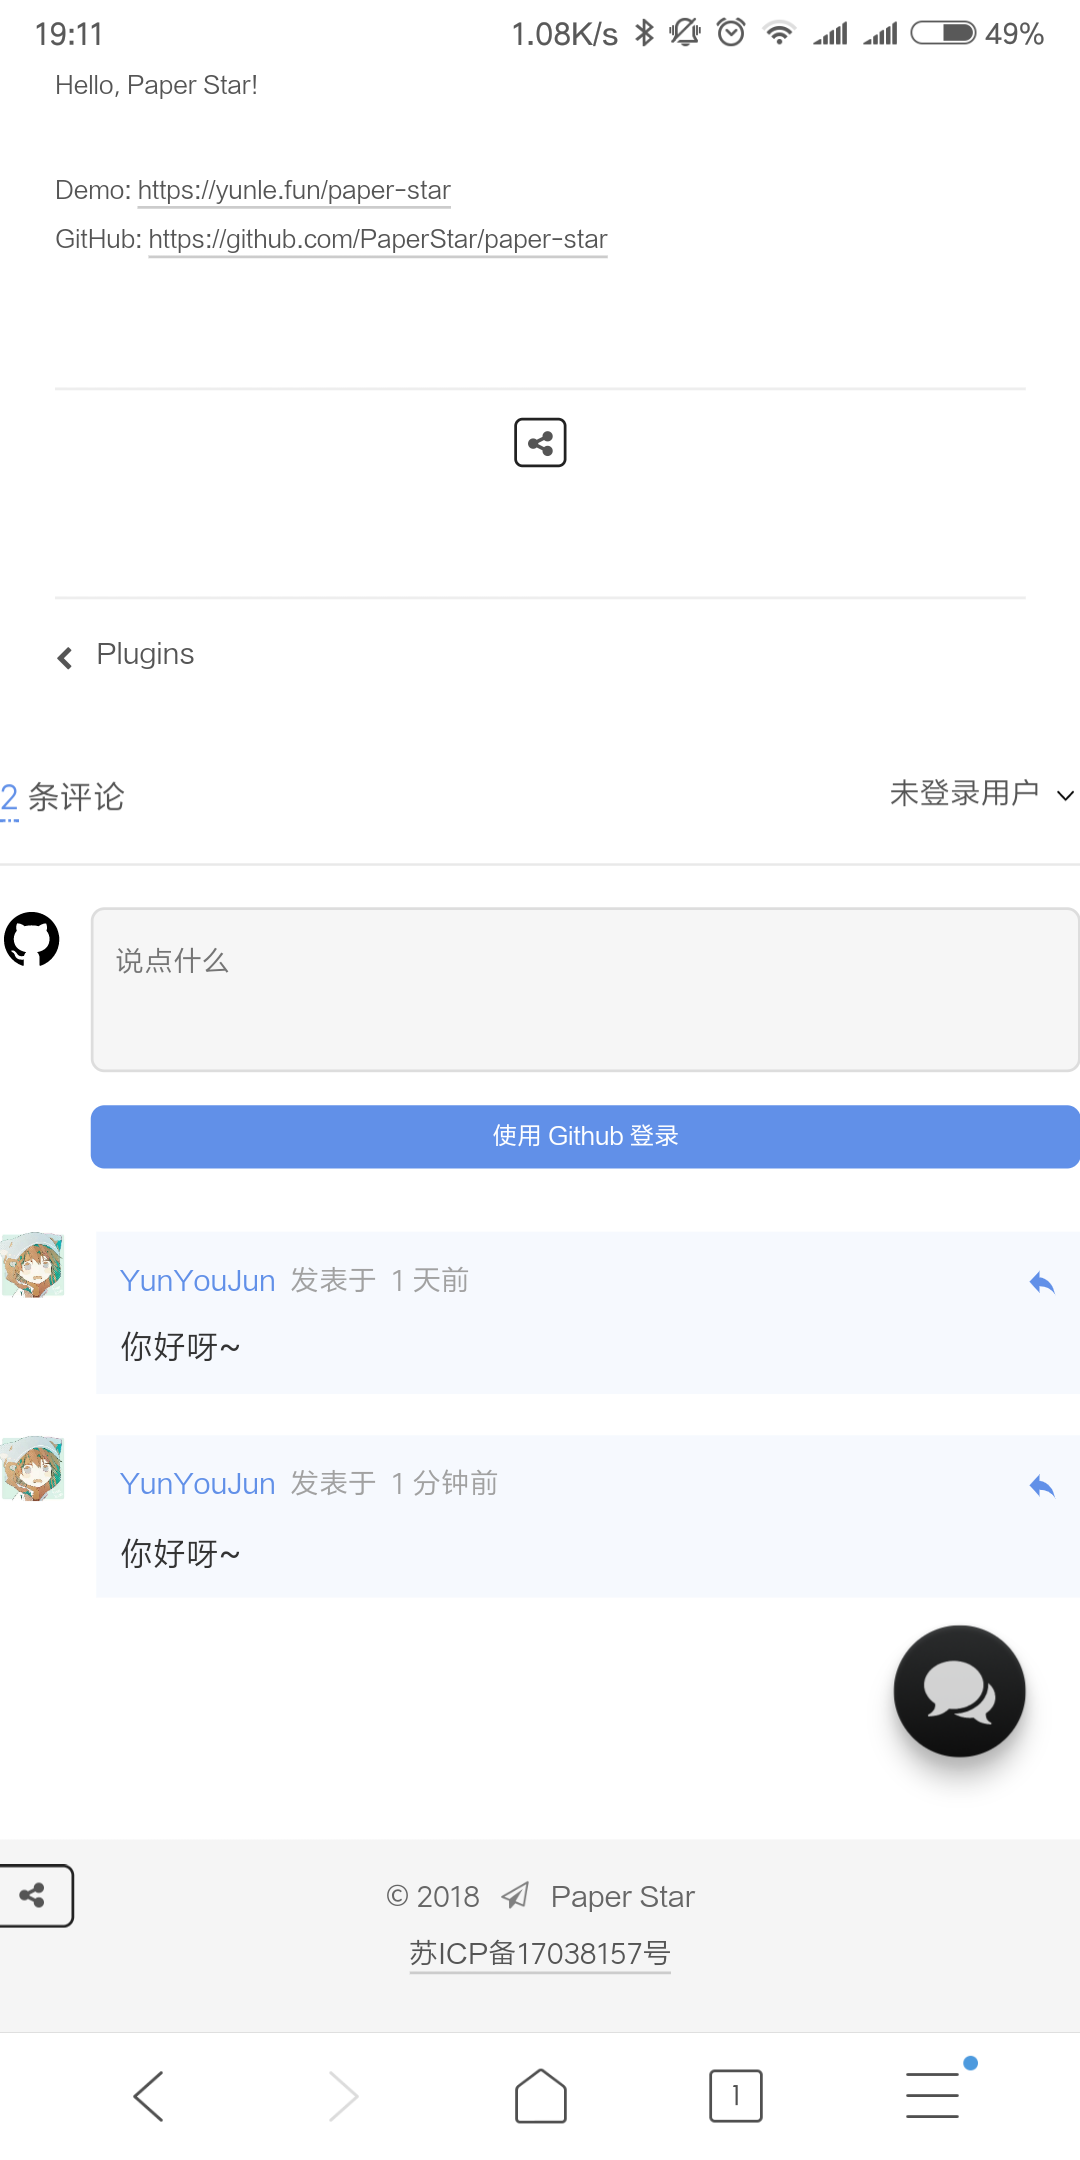
\includegraphics[width=5cm]{show/gameWeb-gitalk}}
  \caption{游戏官网}
  \label{fig:gameWeb}
\end{figure}